% (c) 2012 -2014 Dimitrios Vrettos - d.vrettos@gmail.com
% (c) 2014 Claudio Carboncini - claudio.carboncini@gmail.com
% (c) 2014 Daniele Zambelli - daniele.zambelli@gmail.com

\section{Esercizi}

\subsection{Esercizi dei singoli paragrafi}

%\subsubsection*{2.3 - Confronto di numeri relativi}
\subsubsection*{\numnameref{sec:02_confronto}}

% % Confronto di numeri relativi

\begin{esercizio}
 \label{ese:2.1}
Riscrivi in ordine crescente (dal più piccolo al più grande) i seguenti numeri 
relativi:
\[+11\qquad-3\qquad0\qquad+2\qquad-5\qquad-7\qquad+1\]
\end{esercizio}

\begin{esercizio}
 \label{ese:2.2}
Riscrivi in ordine decrescente (dal più grande al più piccolo) i seguenti numeri 
relativi:
\[-5\qquad-2\qquad+3\qquad-1\qquad0\qquad+7\qquad-9\qquad+13\qquad-21\]
\end{esercizio}

\begin{esercizio}
 \label{ese:2.3}
Disponi sulla retta orientata i seguenti numeri relativi$-3; +2; +5; -7; -5; -1; 
+3$
\begin{center}
 % (c) 2012 Dimitrios Vrettos - d.vrettos@gmail.com
% Esercizio 2.3
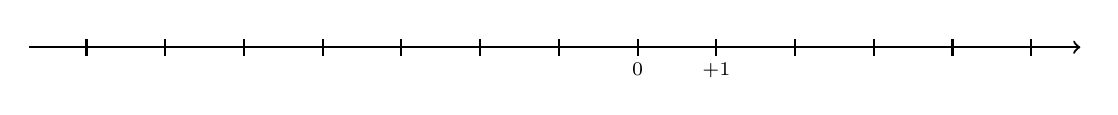
\begin{tikzpicture}

\begin{scope}[thick,font=\scriptsize]
  \draw[->] (-220pt,0)  - -  (160pt,0) node[above]{$\insZ$};	
    \foreach \n in {-7,-6,...,-1}{%
      \draw (\n,-3pt) -- (\n,3pt)   node [below=5pt] {};		
    }

    \foreach \m in {2,3,...,5}{%
      \draw (\m,-3pt) -- (\m,3pt) node [below=5pt]{};
    }

    \foreach \x in {1}{%
      \draw (\x,-3pt) -- (\x,3pt) node [below=5pt]{+$\x$};
    }
    
    \foreach \y in {0}{%
      \draw (\y,-3pt) -- (\y,3pt) node [below=5pt]{$\y$};
    }
\end{scope}
\end{tikzpicture}

\end{center}

\end{esercizio}

\begin{esercizio}
 \label{ese:2.4}
Per ciascuno dei seguenti numeri relativi scrivi il valore assoluto.
\begin{multicols}{3}
\begin{enumeratea}
 \item $|+3|=\ldots$
 \item $|-5|=\ldots$
 \item $|-1|=\ldots$
 \item $|+10|=\ldots$
 \item $|-11|=\ldots$
 \item $|+7|=\ldots$
\end{enumeratea}
\end{multicols}
\end{esercizio}

 \begin{esercizio}
\label{ese:2.5}
Scrivi tra le seguenti coppie di numeri relativi il simbolo corretto tra ``$>$'' 
e ``$(<)$''.
\begin{multicols}{3}
 \begin{enumeratea}
 \item $ -5\ldots-2~$
 \item $ -3\ldots+5~$
 \item $ -2\ldots+2~$
 \item $ -5\ldots0~$
 \item $ -3\ldots-5~$
 \item $ -1\ldots+1~$
 \item $ +3\ldots-3~$
 \item $ -1\ldots-5~$
 \item $~0\ldots+1~$
 \item $ +3\ldots0~$
 \item $~0\ldots -2$
 \item $ +7\ldots +2$
 \item $ -11\ldots-101~$
 \item $ +100\ldots-99~$
 \item $ -101\ldots+110~$
%  \item $ -1010\ldots-1100~$
%  \item $ +324\ldots -282$
%  \item $ -714\ldots -851$
 \end{enumeratea}
\end{multicols}
\end{esercizio}

%\subsubsection*{2.4 - Le operazioni con i numeri relativi}
\subsubsection*{\numnameref{sec:02_operazioni}}

% % Addizione

\begin{esercizio}
 \label{ese:2.6}
Esegui le seguenti addizioni di numeri relativi.
 \begin{multicols}{3}
 \begin{enumeratea}
 \item $(+3)+(+2) =~$
 \item $(-5)+(-5) =~$
 \item $(-3)+(+5) =~$
 \item $(+12)+(+2) =$
 \item $(-2)+(-3) =$
 \item $(-3)+(+13) =$
 \item $(+10)+(-5) =$
 \item $(+1)+(+1) =$
 \item $(-10)+0 =$
 \item $(-4)+(+4) =$
 \item $(+7)+(-6) =$
 \item $(-9)+(-3) =$
 \item $(-101)+(+2) =$
 \item $0+(-9) =$
 \item $(-10)+(+10) =$
 \end{enumeratea}
 \end{multicols}
\end{esercizio}


\begin{esercizio}
 \label{ese:2.7}
Per ognuno dei seguenti numeri relativi scrivi il numero opposto.
 \begin{multicols}{3}
 \begin{enumeratea}
 \item $+3\to\ldots$
 \item $-2\to\ldots$
 \item $+1\to\ldots$
 \item $-11\to\ldots$
 \item $-3\to\ldots$
 \item $+5 \to\ldots$
 \end{enumeratea}
 \end{multicols}
\end{esercizio}

\begin{esercizio}
 \label{ese:2.8}
Completa la seguente tabella.

 \begin{tabular*}{.9\textwidth}{@{\extracolsep{\fill}}*{11}{c}}
 \toprule
~$a$ &$+$1 &$-$2 &0 &$+$2 &$-$3 &$+$3 &$-$1 &$+$4 &$-$5 &$-$10\\
 $b$ &0 &$-$2 &$-$3&$+$1 &$-$5 &$-$3 &$-$10&$-$5 &$+$4 &$+$4 \\
 \midrule
~$a+b$& & & & &	 & & & &	 &\\
 \bottomrule
 \end{tabular*}

\end{esercizio}

% % Sottrazione

\begin{esercizio}
Esegui le seguenti sottrazioni di numeri relativi.
\label{ese:2.9}
\begin{multicols}{3}
\begin{enumeratea}
 \item $(-1)-(+2) =~$
 \item $(-5)-(+3) =~$
 \item $(-2)-(+5) =~$
 \item $(+12)-(+2) =$
 \item $(+1)-(-3) =$
 \item $(-3)-(+1) =$
 \item $(+11)-(-5) =$
 \item $(+21)-(+11) =$
 \item $(-1)-0 =$
 \item $(-3)-(+4) =$
 \item $(+7)-(-2) =$
 \item $(-3)-(-3) =$
 \item $0-(-11) =$
 \item $(-6)-(-6) =$
 \item $(+5)-(-5) =$
\end{enumeratea}
\end{multicols}
\end{esercizio}

\begin{esercizio}
 \label{ese:2.10}
Completa la seguente tabella.

 \begin{tabular*}{.9\textwidth}{@{\extracolsep{\fill}}*{11}{c}}
 \toprule
~$a$ &$-$2 &$-$2 &$-$3 &$+$2 &$-$10 &$+$3 &$-$1 &$-$7 &$+$8 &$-$9\\
 $b$ &0 &$-$3 &$-$3 &$-$5 &$-$5 &$-$1 &$-$10&$-$5 &$+$8 &$+$4 \\
 \midrule
~$a-b$& & & & &	 & & & & &\\
 \bottomrule
 \end{tabular*}

\end{esercizio}

\begin{esercizio}
 \label{ese:2.11}
Completa la seguente tabella.

 \begin{tabular*}{.9\textwidth}{@{\extracolsep{\fill}}*{11}{c}}
 \toprule
~$a$ &$-$2 &$+$2 &$-$1 &$+$2 &$-$10 &$-$5 &$-$1 &$-$7 &$+$8 &$-$9\\
 $b$ &$+$1 &$-$3 &$-$2 &$-$1 &$+$11 &$+$1 &$-$7 &$-$2 &$-$3 &$-$4 \\
 $c$ &$-$3 &$-$5 &$-$6 &$+$1 &$-$1 &$-$2 &$-$2 &$-$5 &$-$3 &$+$2\\
 \midrule
~$a-(b+c)$& & & & &  & & & & &\\
 \bottomrule
 \end{tabular*}

\end{esercizio}

\begin{esercizio}
 \label{ese:2.12}
Completa la seguente tabella.

 \begin{tabular*}{.9\textwidth}{@{\extracolsep{\fill}}*{11}{c}}
 \toprule
 $a$ &$+$1 &$+$2 &$-$2 &$-$3 &$+$4 &$-$5 &$-$1 &$+$6 &$-$7 &$+$10\\
 $b$ &$-$1 &0 &$-$3 &$-$2 &$+$4 &$-$2 &$+$1 &$-$4 &$-$3 &$+$4\\
 $c$ &0 &$-$1 &$+$1 &$-$2 &$+$3 &$-$3 &$+$4 &$-$5 &$+$5 &$-$6\\
 \midrule
 $a-(b+c)$ & & & & & & & & & &\\
 \midrule
 $a-b+c$ & & & & & & & & & &\\
 \midrule
 $a-b-c$ & & & & & & & & & &\\
 \bottomrule
 \end{tabular*}
\end{esercizio}

\begin{esercizio}
 \label{ese:2.13}
Completa la seguente tabella.

 \begin{tabular*}{.9\textwidth}{@{\extracolsep{\fill}}*{11}{c}}
 \toprule
 $a$ &$-$2 &$+$2 &$-$1 &$+$1 &0 &$+$1 &$-$1 &$+$2 &$-$2 &$+$3\\
 $b$ &$-$1 &$+$1 &0 	 &$+$1 &$-$1 &$+$2 &$-$2 &$+$3 &$-$3 &$+$3\\
 \midrule
 $a+b$ & & & & & & & & & &\\
 \midrule
 $-a+b$ & & & & & & & & & &\\
 \midrule
 $-a-b$ & & & & & & & & & &\\
 \midrule
 $-(a+b)$ & & & & & & & & & &\\
 \midrule
 $-(a-b)$ & & & & & & & & & &\\
 \midrule
 $-(-a+b)$ & & & & & & & & & &\\
 \bottomrule
 \end{tabular*}
\end{esercizio}

% % Somma algebrica

\begin{esercizio}
Esegui le seguenti somme algebriche.
 \label{ese:2.14}
 \begin{multicols}{3}
 \begin{enumeratea}
 \item $+3 -1 = +\ldots$
 \item $+2 -3 = -\ldots$
 \item $-5 +2 = -\ldots$
 \item $-2 +2 = \ldots\ldots$
 \item $-5 -2 = \ldots7$
 \item $-3 +5 = \ldots2$
 \item $+8 -0 = \ldots\ldots$
 \item $-9 +0 = \ldots\ldots$
 \item $0 -5 = \ldots\ldots$
 \item $+1 -1 = \ldots\ldots$
 \item $-2 -2 = \ldots\ldots$
 \item $+9 -3 = \ldots6$
 \item $+7 -6 = +\ldots$
 \item $-101 +9 = -\ldots$
 \item $-10 +5 = \ldots~5$
 \end{enumeratea}
 \end{multicols}
\end{esercizio}

\begin{esercizio}
 \label{ese:2.15}
Esegui le seguenti somme algebriche.
\begin{multicols}{3}
 \begin{enumeratea}
 \item $-5 -2 =$
 \item $+3 -4 =$
 \item $-1 +2 =$
 \item $-3 +4 =$
 \item $-6 +7 =$
 \item $-1 -9 =$
 \item $+8 -7 =$
 \item $+2 -1 =$
 \item $-6 +2 =$
 \item $+5 -2 =$
 \item $+4 -3 =$
 \item $+4 +1 =$
 \item $+4 -6 =$
 \item $-10 +5 =$
 \item $-16 -4 =$
 \item $-3 -9 =$
 \item $+14 -7 =$
 \item $-10 -10 =$
 \end{enumeratea}

\end{multicols}

\end{esercizio}

% % Moltiplicazione
\begin{esercizio}
 \label{ese:2.16}
Calcola i seguenti prodotti.
\begin{multicols}{3}
 \begin{enumeratea}
 \item $(+3)\cdot(-2) =-\ldots$
 \item $(-5)\cdot(-2)=+\ldots$
 \item $(+2)\cdot(+4) =\ldots8$
 \item $(+1)\cdot(-1) =\ldots1$
 \item $(+3)\cdot0 = \ldots\ldots$
 \item $(-2)\cdot(-2) =\ldots\ldots$
 \item $0\cdot(-3) = \ldots\ldots$
 \item $(-2)\cdot(+2) =\ldots\ldots$
 \item $(+10)\cdot(-1) =\ldots$

 \end{enumeratea}
\end{multicols}
\end{esercizio}

\begin{esercizio}
 \label{ese:2.17}
Esegui le seguenti moltiplicazioni.
\begin{multicols}{3}
 \begin{enumeratea}
 \item $(+3)\cdot(+1) =$
 \item $(+1)\cdot(-2) =$
 \item $(+3)\cdot(-3) =$
 \item $(-5)\cdot(-1) =$
 \item $(+3)\cdot(-3) =$
 \item $(-2)\cdot(+5) =$
 \item $(-1)\cdot(-7) =$
 \item $(+3)\cdot(+11) =$
 \item $(+1)\cdot(-10) =$
 \item $(-4)\cdot(+3) =$
 \item $(+5)\cdot(-6) =$
 \item $(-3)\cdot(-2) =$
 \end{enumeratea}
\end{multicols}
\end{esercizio}

\begin{esercizio}
 \label{ese:2.18}
Completa la seguente tabella.

 \begin{tabular*}{.9\textwidth}{@{\extracolsep{\fill}}*{11}{c}}
 \toprule
$a$ &$-$2 &$+$2 &$-$1 &$+$2 &$-$10 &$-$5 &$-$1 &$-$7 &$+$8 &$-$9\\
 $b$ &$+$1 &$-$3 &$-$2 &$-$1 &$+$11 &$+$1 &$-$7 &$-$2 &$-$3 &$-$4 \\
 \midrule
$a\cdot b$& & & & & & & & & &\\
 \bottomrule
 \end{tabular*}

\end{esercizio}



% % Divisione
\begin{esercizio}
\label{ese:2.19}
 Esegui le seguenti divisioni.
\begin{multicols}{3}
 \begin{enumeratea}
 \item $(+4):(+2) =$
 \item $(+5):(-1) =$
 \item $(+6):(+2) =$
 \item $(+8):(-2) =$
 \item $(-8):(+4) =$
 \item $(-4):(+2) =$
 \item $(-10):(+5) =$
 \item $(+10):(-2) =$
 \item $(-12):(+6) =$
 \item $(-12):(+4) =$
 \item $(+12):(-3) =$
 \item $(-12):(+1) =$
 \end{enumeratea}
 \end{multicols}
\end{esercizio}

\begin{esercizio}
 \label{ese:2.20}
Completa la seguente tabella.

 \begin{tabular*}{.9\textwidth}{@{\extracolsep{\fill}}*{11}{c}}
 \toprule
$a$ &$-$2 &$+$12 &$-$6 &$+$20 &$-$10 &$-$5 &$-$21 &$-$16 &$+$8 &$-$32\\
 $b$ &$+$1 &$-$3 &$-$2 &$-$1 &$-$5 &$+$1 &$-$7 &$-$2 &$-$4 &$-$4 \\
 \midrule
$a:b$& & & & & & & & & &\\
 \bottomrule
 \end{tabular*}

\end{esercizio}

\clearpage
\begin{esercizio}
 \label{ese:2.21}
Completa la seguente tabella.

 \begin{tabular*}{.9\textwidth}{@{\extracolsep{\fill}}*{11}{c}}
 \toprule
 $a$ &0 &$+$2 &$+$1 &$-$4 &$-$6 &$-$8 &$+$10 &$+$12 &$-$14 &$-$16\\
 $b$ &$+$1 &$-$1 &$-$1 &$+$2 &$-$3 &$+$2 &$-$5 &$-$6 &$-$7 &$+$8\\
 \midrule
 $a:b$ & & & & & & & & & &\\
 \midrule
 $-a:b$ & & & & & & & & & &\\
 \midrule
 $-(a:b)$ & & & & & & & & & &\\
 \midrule
 $a:(-b)$ & & & & & & & & & &\\
 \bottomrule
 \end{tabular*}
\end{esercizio}

% % Potenza di un numero relativo
\begin{esercizio}
\label{ese:2.22}
Calcola il valore delle seguenti potenze.
\begin{multicols}{3}
 \begin{enumeratea}
 \item $(+3)^2 =$
 \item $(-1)^2 =$
 \item $(+1)^3 =$
 \item $(-2)^2 =$
 \item $(-2)^3 =$
 \item $(+2)^3 =$
 \item $(-3)^2 =$
 \item $(-3)^3 =$
 \item $(-4)^1 =$
 \item $(+4)^1 =$
 \item $(-4)^2 =$
 \item $(-2)^4 =$
 \item $(-3)^0 =$
 \item $(-1)^5 =$
 \item $(-2)^4 =$
 \end{enumeratea}
 \end{multicols}
\end{esercizio}

\begin{esercizio}
\label{ese:2.23}
 Applica le proprietà delle potenze.
\begin{multicols}{2}
 \begin{enumeratea}
 \item $(-3)^2\cdot(-3)^3 = (-3)^{\ldots}$
 \item $(-2)^4\cdot(-2)^5 = (-2)^{\ldots}$
 \item $(-5)\cdot(-5)^2 = (-5)^{\ldots}$
 \item $(-10)^2\cdot(-5)^2 = (\ldots \ldots)^2$
 \item $(-3)^4:(-3)^2 = (-3)^{\ldots}$
 \item $(-7)^3:(-7)^3=(-7)^{\ldots}$
 \item $(-2)^4:(-2)^2=(-2)^{\ldots}$
 \item $(-6)^4:(+2)^4=(\ldots \ldots)^4$
 \item $\big[(-3)^2\big]^3 = (-3)^{\ldots}$
 \item $\big[(-5)^2\big]^3=(+5)^{\ldots}$
 \item $(-3)^3\cdot(+3)^3 = \ldots$
 \item $(-8)^2:(-4)^2= \ldots$
 \item $\big[(-7)^2\big]^3: (-7)^3 =\ldots$
 \item $\big[(-3)^3\big]^2: (-3)^4=\ldots$
 \end{enumeratea}
 \end{multicols}
\end{esercizio}


\begin{esercizio}
 \label{ese:2.24}
Completa la seguente tabella.

 \begin{tabular*}{.9\textwidth}{@{\extracolsep{\fill}}*{11}{c}}
 \toprule
 $a$ &$-$2 &$+$1 &$+$2 &$-$1 &$+$3 &$-$3 &$-$4 &$-$2 &$+$2 &$-$3\\
 $b$ &1 &3 &2 &4 &2 &3 &2 &4 &5 &2\\
 \midrule
 $a^b$ & & & & & & & & & &\\
 \bottomrule
 \end{tabular*}
\end{esercizio}


\begin{esercizio}
 \label{ese:2.25}
Completa la seguente tabella.

 \begin{tabular*}{.9\textwidth}{@{\extracolsep{\fill}}*{11}{c}}
 \toprule
~$a$ &$-$2 &$+$12 &$-$6 &$+$20 &$-$10 &$-$5 &$-$21 &$-$16 &$+$8 &$-$12\\
 $b$ &$+$1 &$-$3 &$-$2 &$-$1 &$-$5 &$+$1 &$+$19 &$-$14 &$-$4 &$-$8 \\
 \midrule
~$(a-b)^2$& & & & & & & & & &\\
 \bottomrule
 \end{tabular*}

\end{esercizio}

\begin{esercizio}
 \label{ese:2.26}
Completa la seguente tabella.

 \begin{tabular*}{.9\textwidth}{@{\extracolsep{\fill}}*{11}{c}}
 \toprule
~$a$ &$-$1 &$-$2 &$+$3 &0 &$+$1 &$+$2 &$-$4 &$+$5 &$-$5 &$-$3\\
 \midrule
~$a^2$& & & & & & & & &	 &\\
 \midrule
~$-a^2$& & & & & & & & &	 &\\
 \midrule
~$-(-a)^2$& & & & & & & & &	 &\\
 \bottomrule
 \end{tabular*}

\end{esercizio}

\begin{esercizio}
 \label{ese:2.27}
Completa la seguente tabella.

 \begin{tabular*}{.9\textwidth}{@{\extracolsep{\fill}}*{11}{c}}
 \toprule
$a$ &$-$2 &$-$3 &$+$3 &$-$1 &0 &$-$2 &$-$4 &$-$3 &$+$4 &$+$5\\
 $b$ &0 &$+$1 &$-$1 &$-$2 &$+$2 &$-$3 &$+$2 &$-$2 &$-$3 &$-$5\\
 \midrule
$a\cdot b$& & & & & & & & & &\\
 \midrule
$-a\cdot b$& & & & & & & & & &\\
 \midrule
$(-a)\cdot(-b)$& & & & & & & & & &\\
 \midrule
$-a^2	\cdot b$& & & & & & & & & &\\
 \bottomrule
 \end{tabular*}

\end{esercizio}

% % Proprietà distributiva della moltiplicazione rispetto all'addizione
\begin{esercizio}
 \label{ese:2.28}
Completa la seguente tabella.

 \begin{tabular*}{.9\textwidth}{@{\extracolsep{\fill}}*{11}{c}}
 \toprule
$a$ &$-$2 &$+$2 &$-$1 &$+$2 &$-$10 &$-$5 &$-$1 &$-$7 &$+$8 &$-$9\\
 $b$ &$+$1 &$-$3 &$-$2 &$-$1 &$+$11 &$+$1 &$-$7 &$-$2 &$-$3 &$-$4 \\
 $c$ &$-$3 &$-$5 &$-$6 &$+$1 &$-$1 &$-$2 &$-$2 &$-$5 &$-$3 &$+$2\\
 \midrule
$(a+b)\cdot c$& & & & & & & & & &\\
 \bottomrule
 \end{tabular*}

\end{esercizio}

\begin{esercizio}
 \label{ese:2.29}
Completa la seguente tabella.

 \begin{tabular*}{.9\textwidth}{@{\extracolsep{\fill}}*{11}{c}}
 \toprule
$a$ &$-$2 &$+$12 &$-$6 &$+$20 &$-$10 &$-$5 &$-$21 &$-$16 &$+$8 &$-$12\\
 $b$ &$+$1 &$-$3 &$-$2 &$-$1 &$-$5 &$+$1 &$+$19 &$-$14 &$-$4 &$-$8 \\
 \midrule
$(a+b)(a-b)$
 \end{tabular*}

\end{esercizio}

\begin{esercizio}
 \label{ese:2.30}
Completa la seguente tabella.

 \begin{tabular*}{.9\textwidth}{@{\extracolsep{\fill}}*{11}{c}}
 \toprule
$a$ &$+$1 &0 &$-$1 &$+$2 &$-$2 &0 &$+$3 &$-$3 &$+$4 &$-$10\\
 $b$ &$+$2 &0 &$+$1 &$-$1 &$-$2 &$-$3 &$+$2 &$+$3 &$+$4 &$+$8\\
 $c$ &$+$3 &$+$1 &$+$1 &$-$2 &$-$2 &$+$3 &$-$2 &0 &0 &$+$2\\
 \midrule
$-2a+(b-c)$& & & & & & & & & &\\
 \bottomrule
 \end{tabular*}

\end{esercizio}


\subsection{Esercizi riepilogativi}

\begin{esercizio}
In quali delle seguenti situazioni è utile ricorrere ai numeri relativi?
 \begin{enumeratea}
 \item misurare la temperatura;
 \item contare le persone;
 \item esprimere la data di nascita di un personaggio storico;
 \item esprimere l'età di un personaggio storico;
 \item indicare il saldo attivo o passivo del conto corrente;
 \item indicare l'altezza delle montagne e le profondità dei mari.
 \end{enumeratea}
\end{esercizio}

% \clearpage
\begin{esercizio}
La somma di due numeri relativi è sicuramente positiva quando:
 \begin{multicols}{2}
 \noindent
 \boxA\enspace i due numeri sono concordi.\\
 \boxB\enspace i due numeri sono discordi.\\
 \boxC\enspace i due numeri sono entrambi positivi.\\
 \boxD\enspace i due numeri sono entrambi negativi.
 \end{multicols}
\end{esercizio}

\begin{esercizio}
La somma di due numeri relativi è sicuramente negativa quando:
 \begin{multicols}{2}
 \noindent
 \boxA\enspace i due numeri sono concordi.\\
 \boxB\enspace i due numeri sono discordi.\\
 \boxC\enspace i due numeri sono entrambi positivi.\\
 \boxD\enspace i due numeri sono entrambi negativi.
 \end{multicols}
\end{esercizio}

\begin{esercizio}
Il prodotto di due numeri relativi è positivo quando (più di una risposta 
possibile):
 \begin{multicols}{2}
 \noindent
 \boxA\enspace i due numeri sono concordi.\\
 \boxB\enspace i due numeri sono discordi.\\
 \boxC\enspace i due numeri sono entrambi positivi.\\
 \boxD\enspace i due numeri sono entrambi negativi.
 \end{multicols}
\end{esercizio}

\begin{esercizio}
Il prodotto di due numeri relativi è negativo quando:
 \begin{multicols}{2}
 \noindent
 \boxA\enspace i due numeri sono concordi.\\
 \boxB\enspace i due numeri sono discordi.\\
 \boxC\enspace i due numeri sono entrambi positivi.\\
 \boxD\enspace i due numeri sono entrambi negativi.
 \end{multicols}
\end{esercizio}

\begin{esercizio}
Quali delle seguenti affermazioni sono vere?
\TabPositions{12cm}
\begin{enumeratea}
 \item ogni numero relativo è minore di zero \tab\boxV\quad\boxF
 \item la somma di due numeri discordi è zero \tab\boxV\quad\boxF
 \item il cubo di un numero intero relativo è sempre negativo 
\tab\boxV\quad\boxF
 \item la somma di due numeri opposti è nulla \tab\boxV\quad\boxF
 \item il quoziente di due numeri opposti è l'unità \tab\boxV\quad\boxF
 \item il quoziente di due numeri concordi è positivo \tab\boxV\quad\boxF
 \item il prodotto di due numeri opposti è uguale al loro quadrato 
\tab\boxV\quad\boxF
 \item il doppio di un numero intero negativo è positivo \tab\boxV\quad\boxF
 \item la somma di due interi concordi è sempre maggiore di ciascun addendo 
\tab\boxV\quad\boxF
 \item il quadrato dell'opposto di un intero è uguale all'opposto del suo 
quadrato \tab\boxV\quad\boxF
\end{enumeratea}
\end{esercizio}

\begin{esercizio}
Inserisci l'operazione corretta per ottenere il risultato.
 \begin{multicols}{3}
 \begin{enumeratea}
 \item $(+2)\ldots(-1) = -2$
 \item $(-10)\ldots(+5) = -2$
 \item $(-18)\ldots(-19) = +1$
 \item $(+15)\ldots(-20) = -5$
 \item $(-12)\ldots(+4) = -3$
 \item $(-4)\ldots0 =~0$
 \item $(+1)\ldots(+1) =~0$
 \item $(+5)\ldots(-6) = +11$
 \item $-8\ldots(-2) = +16$
 \end{enumeratea}
 \end{multicols}
\end{esercizio}


\begin{esercizio}
Inserisci il numero mancante.
 \begin{multicols}{3}
 \begin{enumeratea}
 \item $+5 + (\ldots\ldots) = -5$
 \item $-8 + (\ldots\ldots) = -6$
 \item $+7 - (\ldots\ldots) =~0$
 \item $0 - (\ldots\ldots) = -2$
 \item $+3\cdot (\ldots\ldots) = -3$
 \item $-5\cdot (\ldots\ldots) =~0$
 \item $(+16): (\ldots\ldots) = -2$
 \item $(-6): (\ldots\ldots) = -1$
 \item $(-10): (\ldots\ldots) = +5$
 \end{enumeratea}
 \end{multicols}
\end{esercizio}

\begin{esercizio}
 Scrivi tutti i numeri:
 \begin{enumeratea}
 \item interi relativi che hanno valore assoluto minore di~5;
 \item interi relativi il cui prodotto è~$-12$
 \item interi negativi maggiori di~$-5$
 \end{enumeratea}
\end{esercizio}

\begin{esercizio}
Inserisci ``$+$'' o ``$-$'' in modo da ottenere il numero più grande possibile:
 \[-3\ldots(-3)\ldots3\ldots(-6).\]
\end{esercizio}

\begin{esercizio}
Inserisci le parantesi in modo da ottenere il risultato indicato.
 \begin{enumeratea}
 \item $-5 \cdot +3-1+2=-20$
 \item $-5+2\cdot-1+2=+5$
 \item $-5+7-3\cdot 2=+3$
 \item $-1\cdot +3-5\cdot -1-2=+12$
 \item $+1-1\cdot 1 -1+3-2\cdot -3-2=+5$
 \end{enumeratea}
\end{esercizio}

\begin{esercizio}[\Ast]
Calcola il valore delle seguenti espressioni.
 \begin{enumeratea}
 \item $-5+7+4-9$
 \item $+1-1+1-1+1-1+1$
 \item $+1-2+3-4+5-6$
 \item $+1-2+2-3+3-4+5-6+6-7+7-8+8-9+9-10$
 \item $(-3+10)-(2-3)$
 \end{enumeratea}
\end{esercizio}

\begin{esercizio}[\Ast]
Calcola il valore delle seguenti espressioni.
 \begin{enumeratea}
 \item $(+5-2-1)+(+2+4+6)$
 \item $(-5+7-9)+(+1-2+3)-(+4-6+8)$
 \item $+4-3-[+2-1-(8-3)-(-5-2)]-(2+3)$
 \item $-2+(-5+1)+(-7+4)-2 \cdot (-6+1)$
 \item $15-9 \cdot (-14+12)+8 \cdot (-3+6)+ 5 \cdot(-3+1)$
 \end{enumeratea}
\end{esercizio}

\begin{esercizio}[\Ast]
Calcola il valore delle seguenti espressioni.
 \begin{enumeratea}
 \item $(50-36-25)\cdot (-15+5+20)-10\cdot (-3-7)$
 \item $[+3-(10-5+25)]\cdot [-16+5-(-2-14)]:(9+6)$
 \item $20:(+15-5)-30:(-10+5)+40:(15-20)$
 \item $18:(-3)+6\cdot [1-5\cdot (-2+4)+3]: (-6)$
 \item $3\cdot 4-3\cdot [18:(-2)-17+(14-26+5)\cdot 3-12]+[16-1\cdot 
(-1-3+5)-37+16]$
\end{enumeratea}
\end{esercizio}

\begin{esercizio}[\Ast]
Calcola il valore delle seguenti espressioni e indica dove puoi applicare le 
proprietà delle potenze.
\TabPositions{3.5cm}
\begin{enumeratea}
 \item $100:2+3^2 -2^2\cdot 6$ \tab Hai applicato le proprietà delle 
potenze?\enspace\dotfill
 \item $2^7:~2^3 -2^2$ \tab Hai applicato le proprietà delle 
potenze?\enspace\dotfill
 \item $30-5\cdot 3 -7\cdot 2^2 -2$ \tab Hai applicato le proprietà delle 
potenze?\enspace\dotfill
 \item $(3^2 +4^2) -(-3-4)^2$ \tab Hai applicato le proprietà delle 
potenze?\enspace\dotfill
\end{enumeratea}
\end{esercizio}

\begin{esercizio}[\Ast]
Calcola il valore delle seguenti espressioni e indica dove puoi applicare le 
proprietà delle potenze.
\TabPositions{5.5cm}
\begin{enumeratea}
 \item $5\cdot 5^3\cdot 5^4: \big(5^2\big)^3 +5$ \tab Hai applicato le proprietà 
delle potenze?\enspace\dotfill
 \item $32^5:~16^4 +(-2)^9$ \tab Hai applicato le proprietà delle 
potenze?\enspace\dotfill
 \item $\big(3^4\cdot 3^3:~3^6\big)^2 +(7^2-5^2):2^2$ \tab Hai applicato le 
proprietà delle potenze?\enspace\dotfill
 \item $\big(3\cdot 2^2 -10\big)^4\cdot (3^3+2^3):7-10\cdot 2^3$ \tab Hai 
applicato le proprietà delle potenze?\enspace\dotfill
\end{enumeratea}
\end{esercizio}

\begin{esercizio}[\Ast]
Calcola il valore delle seguenti espressioni.
 \begin{enumeratea}
 \item $-5\cdot(12-3+4)-2\cdot\big[3-16:(-2+4)\big]^2$
 \item $\big[-3+(-5)\cdot(-1)\big]^3+\big[-4-(1-2)\big]^2$
 \item $\big[2\cdot(-3)^2+2\cdot(-3)\cdot(-2)\big]^2:\big[2^4-3\cdot(+6)\big]^2$
 \item 
$\big[3\cdot(-1)^2-3\cdot(-3)\cdot(-3)\big]^3:\big[2^2+5\cdot(-2)^2\big]^3$
 \end{enumeratea}
\end{esercizio}

\begin{esercizio}[\Ast]
Calcola il valore delle seguenti espressioni.
 \begin{enumeratea}
 \item $(-3)^2\cdot(4-1)^5:[(-4)^3:(2^5)-3^3:(-3)^3]$
 \item $[-(-2)\cdot2+(-10)^2:(-5)^2]\cdot[3-5+2\cdot(-3)^2-5]$
 \item $13-3-4\cdot(-2)^2-5^3:5^2+3\cdot(2^3-3^2)-6:(-3)-(4-7+3)^4$
 \item $-1-3\cdot(-3)^2-4^3:4^2+(-3-3)\cdot(2^2+3^2)-(-12):(-3)$
 \end{enumeratea}
\end{esercizio}

\begin{esercizio}[\Ast]
Calcola il valore delle seguenti espressioni.
 \begin{enumeratea}
 \item $[10-6\cdot(-2)^2]:(-7)+(3^2:3)\cdot2^3-15:(-3)+[(-3)^3:(-3)^0]$
 \item $|-5+8|-|-11|+(-|+4|\cdot|-2\cdot(+5)|)^2$
 \item $(-29+37)^5\cdot(-5+|23-28|)^7$
 \item $-2\cdot(-2\cdot|-2|)^2-\big(|3-5|\cdot(3-5)\big)^2\cdot(-2)$
 \item $(-1)^3\cdot(-1\cdot|-1|)^2-(|-3-2|\cdot(-5+3))^2\cdot(-2+1)^3$
 \end{enumeratea}
\end{esercizio}
\begin{multicols}{2}
\begin{esercizio}
Traduci in una espressione matematica le seguenti frasi e motivane la verità o 
falsità:
 \begin{enumeratea}
 \item il cubo del quadrato di un numero diverso da zero è sempre positivo;
 \item il quadrato della somma di un numero con il suo opposto è sempre 
positivo;
 \item la differenza tra il triplo di~5 e l'unità è uguale all'opposto di~5;
 \item il prodotto tra il quadrato di un numero negativo e l'opposto dello 
stesso numero 
è uguale all'opposto del suo cubo.
 \end{enumeratea}
\end{esercizio}

\begin{esercizio}
 Sottrarre dal cubo di~$-3$ la somma dei quadrati di~$+$2 e~$-2$ Il risultato è?
\end{esercizio}

\begin{esercizio}
 Sottrarre dalla somma di~$-$15 e~$+$27 il prodotto di~$-$3 e~$+$7.
\end{esercizio}

\begin{esercizio}
 Aggiungere al prodotto di~$-$5 e~$+$3 la somma di~$+$5 e~$-$10.
\end{esercizio}

\begin{esercizio}
 Sottrarre dal prodotto di~$+$7 e~$+$4 la somma di~$+$1 e~$-$8.
\end{esercizio}

\begin{esercizio}
 Moltiplica la somma tra~$-3$ e~$+3$ con la differenza tra~$+3$ e~$-3$
\end{esercizio}

\begin{esercizio}
 Partendo dal pian terreno scendo di~15 gradini, salgo~12 gradini, scendo di~7
gradini e risalgo di~8. A che punto mi trovo rispetto al pian terreno?
\end{esercizio}

\begin{esercizio}
 Giocando a carte contro due avversari nella prima partita ho vinto~50 gettoni 
con il primo giocatore e perso~60
gettoni con il secondo giocatore, nella seconda partita ho perso~30 gettoni con 
il primo e vinto~10 gettoni
con il secondo. Quanti gettoni ho vinto complessivamente?
\end{esercizio}

% \begin{esercizio}[\Ast]
%  Un polpo congelato è stato appena tolto dal congelatore, la sua temperatura 
% è~$-12$\textdegree;
% viene immerso nell'acqua bollente e la sua temperatura media è aumentata 
% di~6\textdegree.
% A quale temperatura media si trova ora il polpo?
% \end{esercizio}

\begin{esercizio}
 Una lumaca sale su un muro alto~10 metri, di giorno sale di due metri ma di 
notte
scende di un metro. In quanti giorni la lumaca arriva in cima al muro?
\end{esercizio}

% \begin{esercizio}[\Ast]
%  Un termometro segna all'inizio~$-$5\textdegree, poi scende di~3\textdegree, 
% quindi sale di~2\textdegree,
% infine discende di~6\textdegree. Quale temperatura segna alla fine?
% \end{esercizio}
% 
% \begin{esercizio}[\Ast]
%  Il prodotto di due numeri interi relativi è~$+$80, aumentando di~1 il primo 
% numero il
% prodotto è~$+$72. Quali sono i due numeri?
% \end{esercizio}

\begin{esercizio}
 Il prodotto di due numeri interi relativi è~$+6$, la loro somma è~$-$5. Quali 
sono i due numeri?
\end{esercizio}


\begin{esercizio}
 Determina due numeri relativi aventi come prodotto~$+$12 e come somma~$-$7.
\end{esercizio}

\begin{esercizio}
 Determina due numeri relativi aventi come prodotto~$+12$ e come somma~$-7$
\end{esercizio}

\begin{esercizio}
 Determina due numeri relativi aventi come prodotto~$+2$ e come somma~$+1$
\end{esercizio}

\begin{esercizio}
 Determina due numeri relativi aventi come prodotto~$+10$ e come somma~$-3$
\end{esercizio}

\begin{esercizio}
 Determina due numeri relativi aventi come prodotto~$+14$ e come somma~$-9$
\end{esercizio}

\begin{esercizio}
 Determina due numeri relativi aventi come prodotto~$-15$ e come somma~$-8$
\end{esercizio}

% \begin{esercizio}
%  Determina due numeri relativi aventi come prodotto~$-7$ e come somma~$+6$
% \end{esercizio}
\end{multicols}
% \subsection{Risposte}

% \paragraph{2.42.}
% a)~$-3$,\quad b)~$+1$,\quad c)~$-3$,\quad d)~$-8$,\quad e)~$+8$
% 
% \paragraph{2.43.}
% a)~$+14$,\quad b)~$-11$,\quad c)~$-7$,\quad d)~$+1$,\quad e)~$+47$
% 
% \paragraph{2.44.}
% a)~$-10$,\quad b)~$-9$,\quad c)~$0$,\quad d)~$0$,\quad e)~$+183$
% 
% \paragraph{2.45.}
% a)~$+35$,\quad b)~$+12$,\quad c)~$-15$,\quad d)~$-24$
% 
% \paragraph{2.46.}
% a)~$+30$,\quad b)~$0$,\quad c)~$+15$,\quad d)~$0$
% 
% \paragraph{2.47.}
% a)~$-115$,\quad b)~$+17$,\quad c)~$+225$
% 
% \paragraph{2.48.}
% a)~$-3^7$,\quad b)~$+88$,\quad c)~$-12$
% 
% \paragraph{2.49.}
% a)~$+4$,\quad b)~$+1592$,\quad c)~$0$,\quad d)~$0$
% 
% \paragraph{2.60.}
% $-6$\textdegree.
% 
% \paragraph{2.61.}
% $-10$ $-8$

